
\section{Introducción}
\begin{frame}\frametitle{Los robots de servicio doméstico}
  \begin{columns}
    \begin{column}{0.5\textwidth}
      Son robots pensados para ayudar en tareas comunes del hogar u oficina. Requieren de varias habilidades:
      \begin{itemize}
      \item Interacción humano-robot
      \item Navegación en ambientes dinámicos
      \item Reconocimiento de objetos
      \item Manipulación de objetos
      \item Comportamientos adaptables
      \item Planeación de acciones
      \end{itemize}
    \end{column}
    \begin{column}{0.4\textwidth}
      \centering
      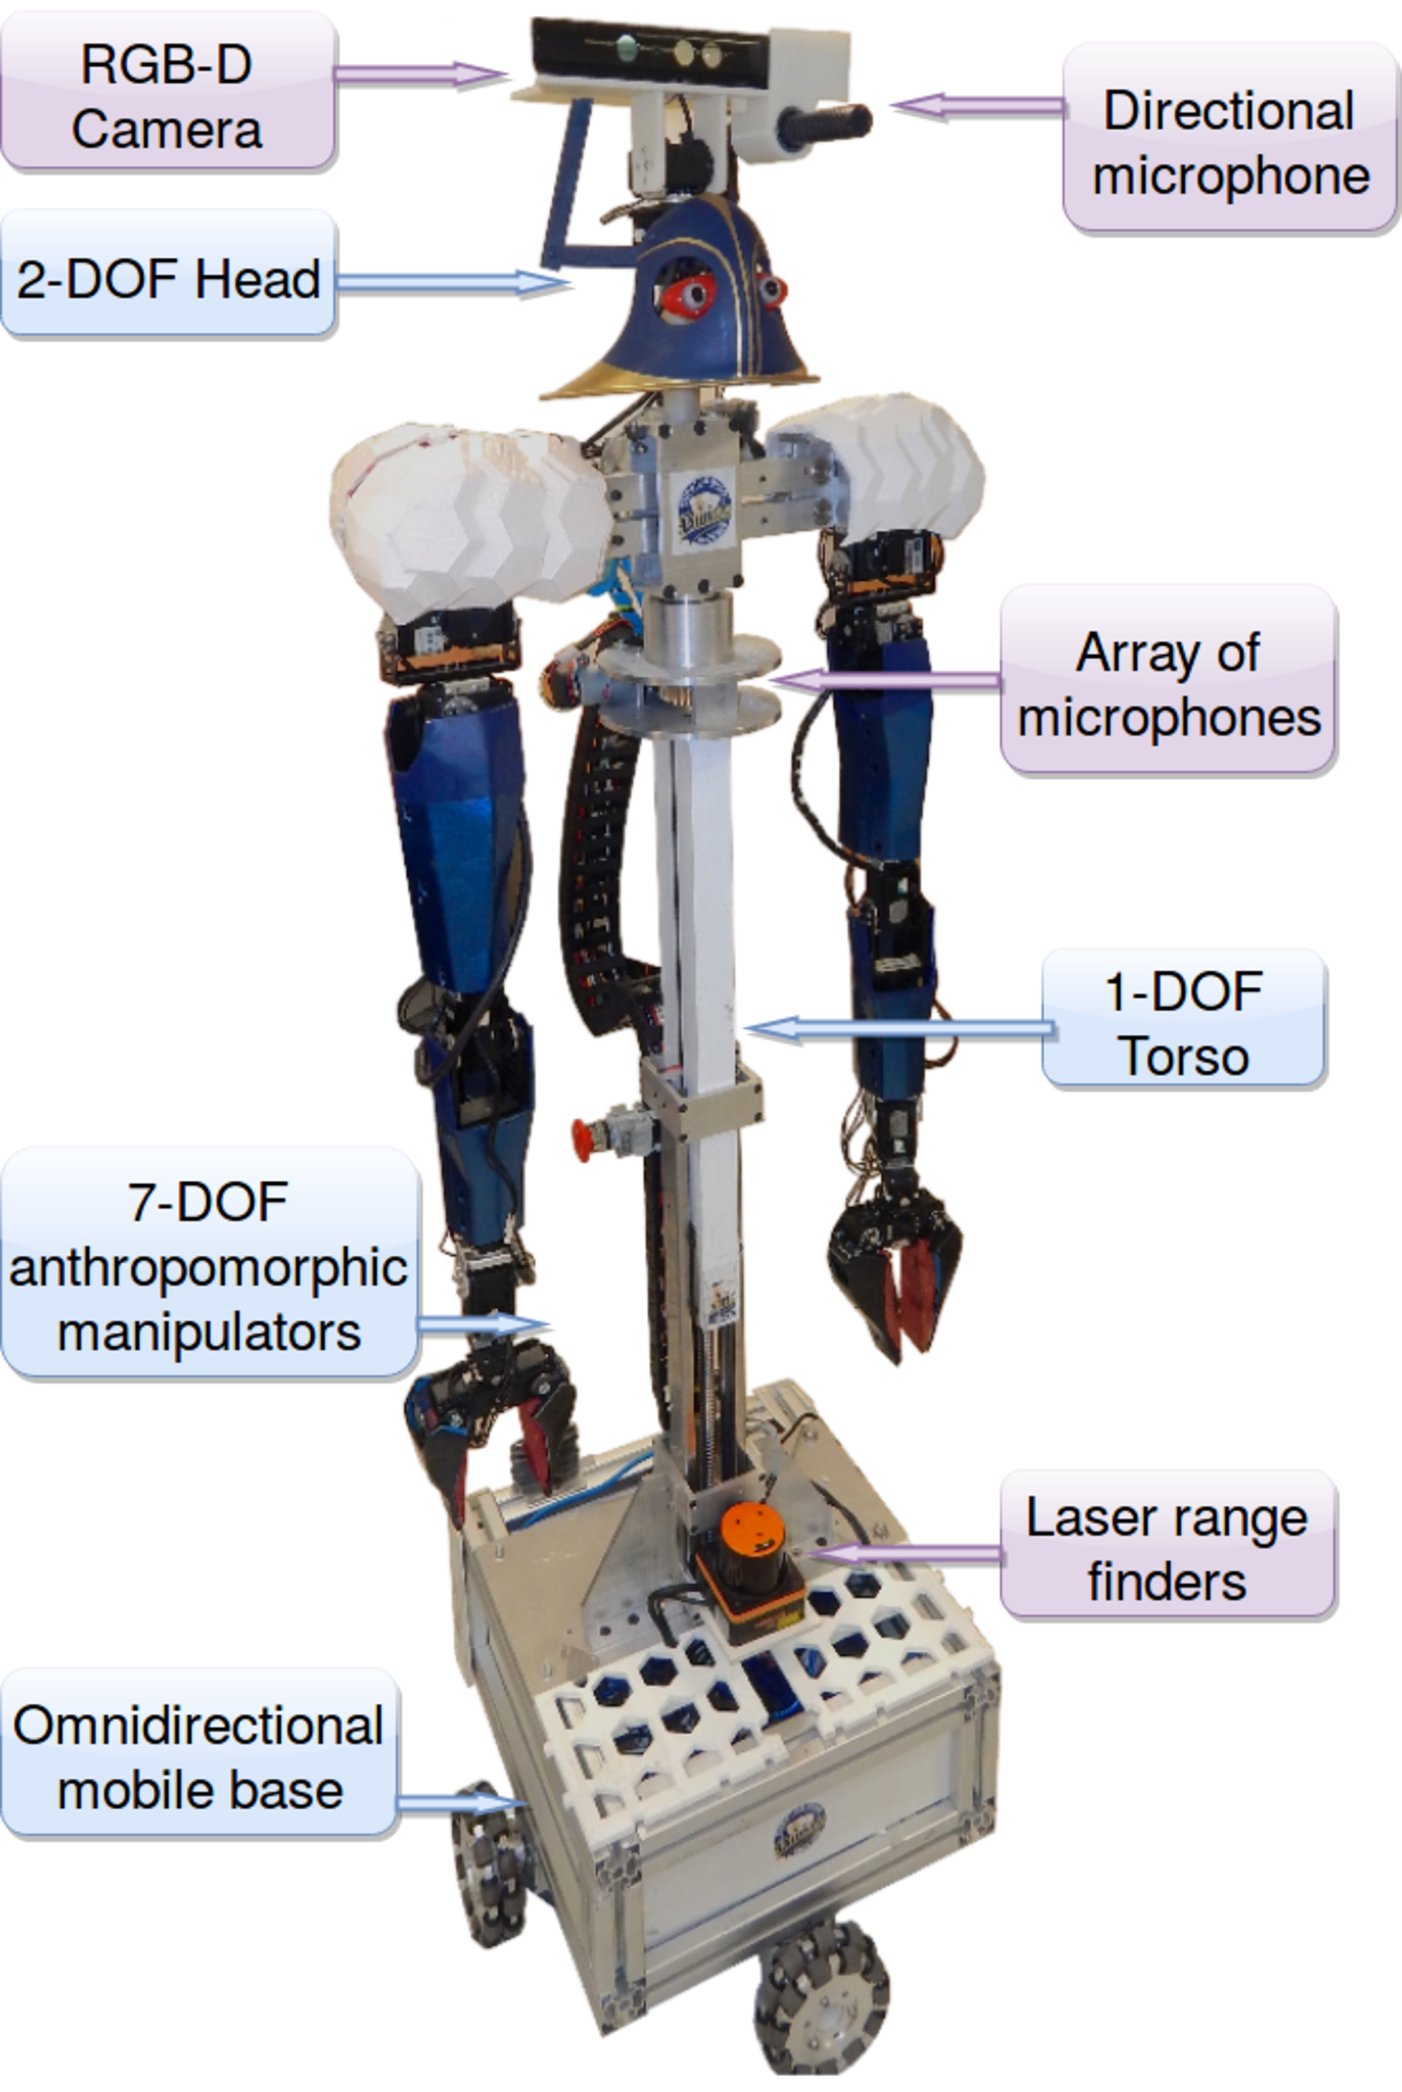
\includegraphics[width=0.9\textwidth]{Figures/Justina.pdf}
    \end{column}
  \end{columns}
\end{frame}

\begin{frame}\frametitle{Hardware necesario: Base móvil}
  \begin{columns}
    \begin{column}{0.5\textwidth}
      \begin{itemize}
      \item De preferencia, debe ser omnidireccional
      \item Turtle Bot (\url{https://www.turtlebot.com/})
      \item Festo Robotino (\url{https://wiki.openrobotino.org/})
      \item DIY: 3 ó 4 motores de corriente directa con ruedas omnidireccionales, 2 tarjetas Roboclaw, baterías de LiPo y chasis de alumnio estructural.
      \end{itemize}
    \end{column}
    \begin{column}{0.5\textwidth}
      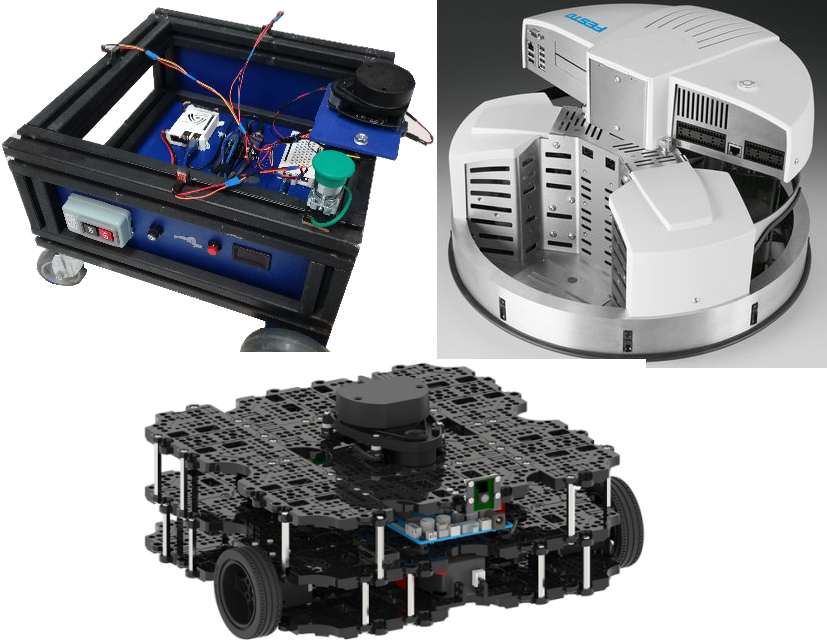
\includegraphics[width=\textwidth]{Figures/Bases.png}
    \end{column}
  \end{columns}
\end{frame}

\begin{frame}\frametitle{Hardware necesario: Cámaras}
  \begin{columns}
    \begin{column}{0.45\textwidth}
      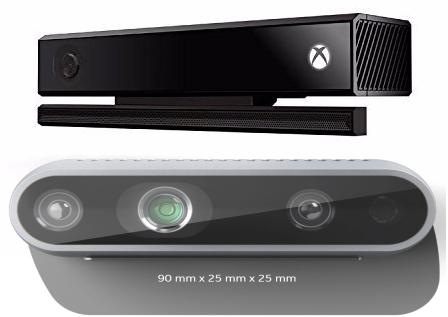
\includegraphics[width=\textwidth]{Figures/Cameras.jpg}
    \end{column}
    \begin{column}{0.5\textwidth}
      \begin{itemize}
      \item Se pueden usar sólo cámaras RGB, pero es altamente recomendable tener información de profundidad.
      \item Kinect (\url{https://github.com/OpenKinect/libfreenect2})
      \item Intel RealSense (\url{https://github.com/IntelRealSense/librealsense})
      \item También se pueden usar cámaras estéreo, pero es mucho más sencillo usar cámaras con luz estructurada.
      \end{itemize}
    \end{column}
  \end{columns}
\end{frame}

\begin{frame}\frametitle{Hardware necesario: Sensor láser}
  \begin{columns}
    \begin{column}{0.5\textwidth}
      \begin{itemize}
      \item Hokuyo (\url{https://www.hokuyo-aut.jp/})
      \item RPLidar (\url{https://www.robotshop.com/en/slamtec.html})
      \item SICK (\url{https://www.sick.com/ag/en/detection-and-ranging-solutions/2d-lidar-sensors/c/g91900})
      \item El paquete \url{http://wiki.ros.org/urg_node} facilita su operación.
      \item Si no se tiene uno, se puede simular a partir de una cámara RGB-D con el paquete \url{http://wiki.ros.org/pointcloud_to_laserscan}.
      \end{itemize}
    \end{column}
    \begin{column}{0.4\textwidth}
      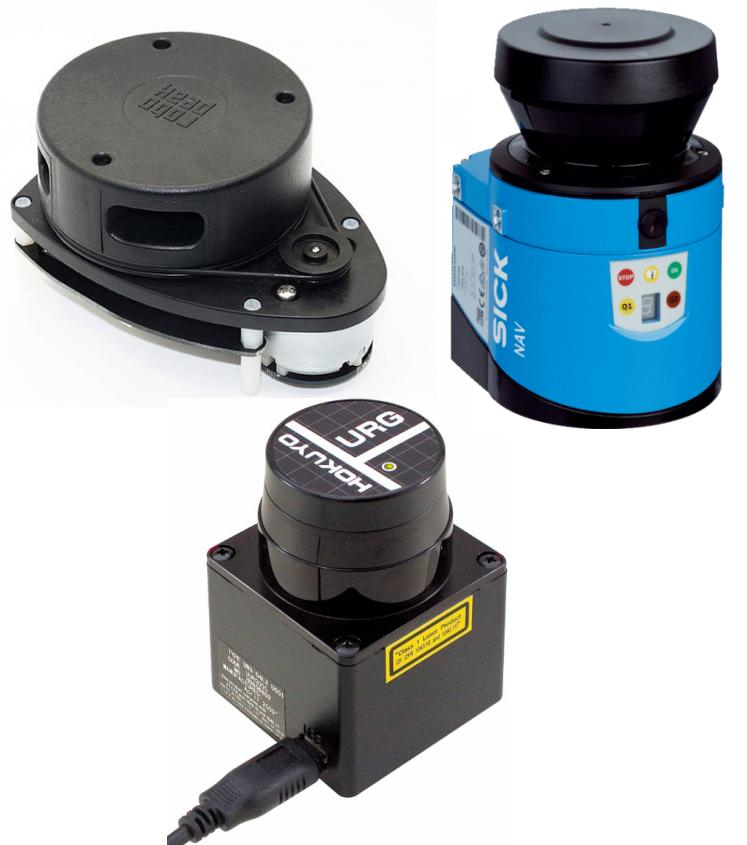
\includegraphics[width=\textwidth]{Figures/lasers.jpg}
    \end{column}
  \end{columns}
\end{frame}

\begin{frame}\frametitle{Hardware necesario: Manipulador}
  \begin{columns}
    \begin{column}{0.4\textwidth}
      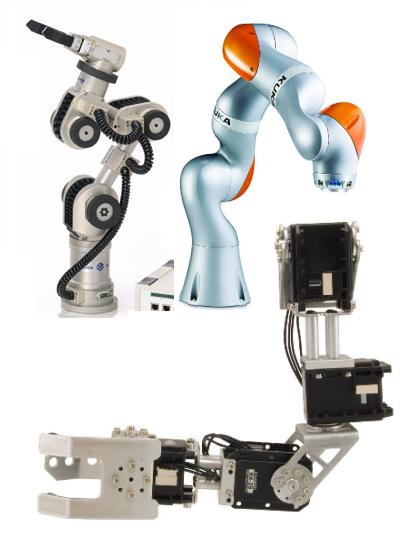
\includegraphics[width=\textwidth]{Figures/arms.jpg}
    \end{column}
    \begin{column}{0.5\textwidth}
      \begin{itemize}
      \item Son recomendables por lo menos 5 DOF.
      \item Kuka LBR iiwa (\url{http://wiki.ros.org/kuka})
      \item Neuronics Katana (\url{http://wiki.ros.org/katana})
      \item DIY: Servomotores y Brackets Dynamixel (\url{http://wiki.ros.org/dynamixel})
      \end{itemize}
    \end{column}
  \end{columns}
\end{frame}
